%===============================================
% INTRODUCTION
%===============================================
\section{Introduction}
\label{sec:intro}
%
This document describes the design and implementation of the Micro Memory Protection Unit (uMPU).
%
For the motivation and architectural principles, refer to the uMPU research paper.
%
An overview of our system highlighting all its components is shown in Figure~\ref{fig:sys_overview}.
%
The final firmware image is composed of multiple software modules that need to be protected from one another.
%
%The software components are installed in separate protection domains.
%
A cross domain linking mechanism (described in Section~\ref{sec:cross_domain_linking}) installs the software modules in separate protection domains.
%
The cross domain linker generates a software jump table that assists the processor in determining the identity of the currently active domain.
%
The Memory Map (described in Section~\ref{sec:memmap}) tracks layout and ownership information for the protected address space.
%
The firmware image interacting with the memory map and hardware enhanced run-time checkers is guaranteed to be memory safe.
%
The detailed description of the architectural extensions is given in Section~\ref{sec:archext}.
%
\begin{figure}[htbp]
   \centering
   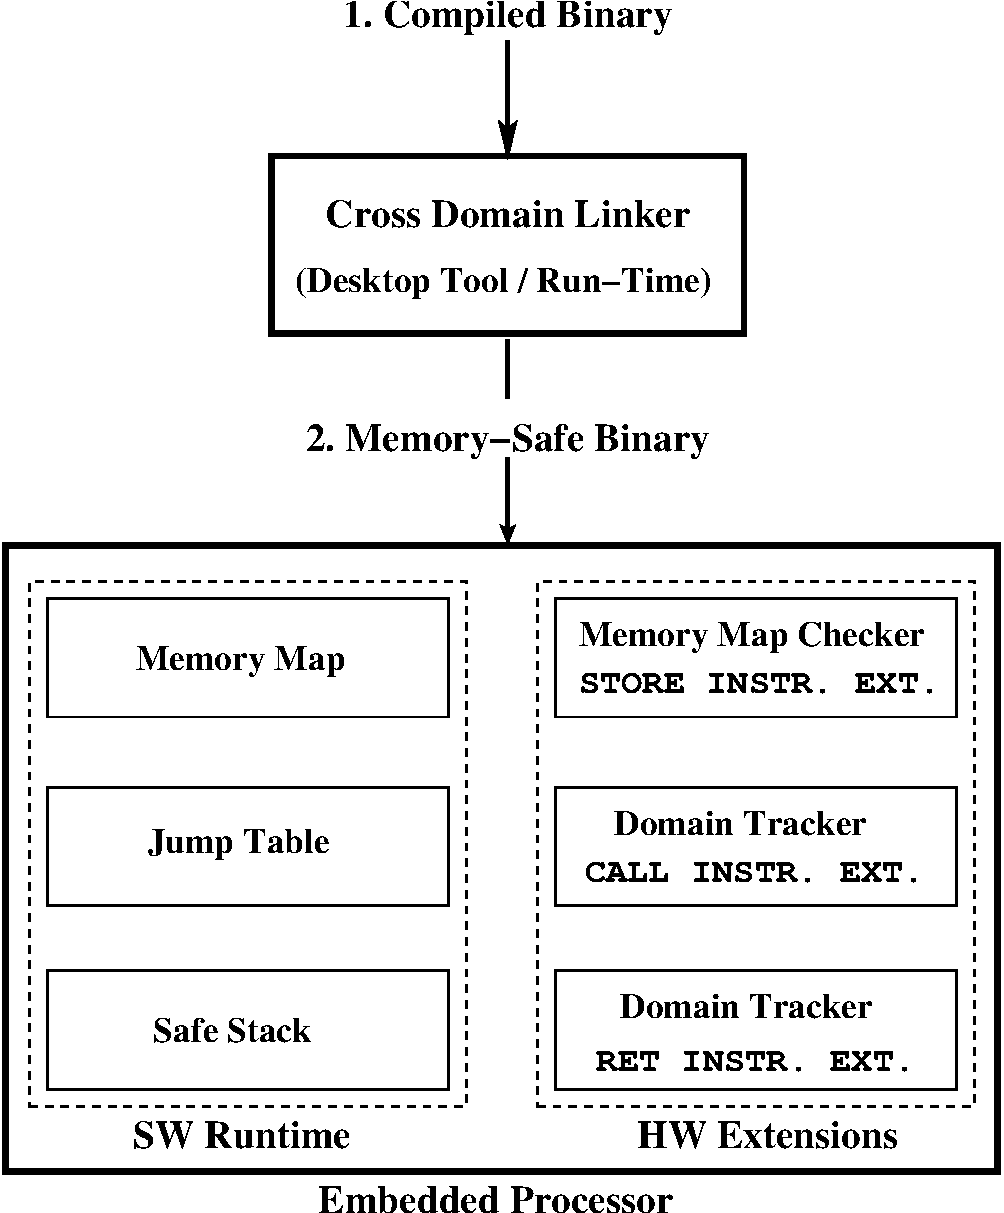
\includegraphics[height = 2.0in, keepaspectratio=true]{figures/sysoverview.pdf} 
   \caption{System Overview}
   \label{fig:sys_overview}
\end{figure}
%
